\documentclass{standalone}

\usepackage{xcolor}
\usepackage{tikz, tkz-euclide}
\usetikzlibrary{arrows}
\usetkzobj{all}

\begin{document}
	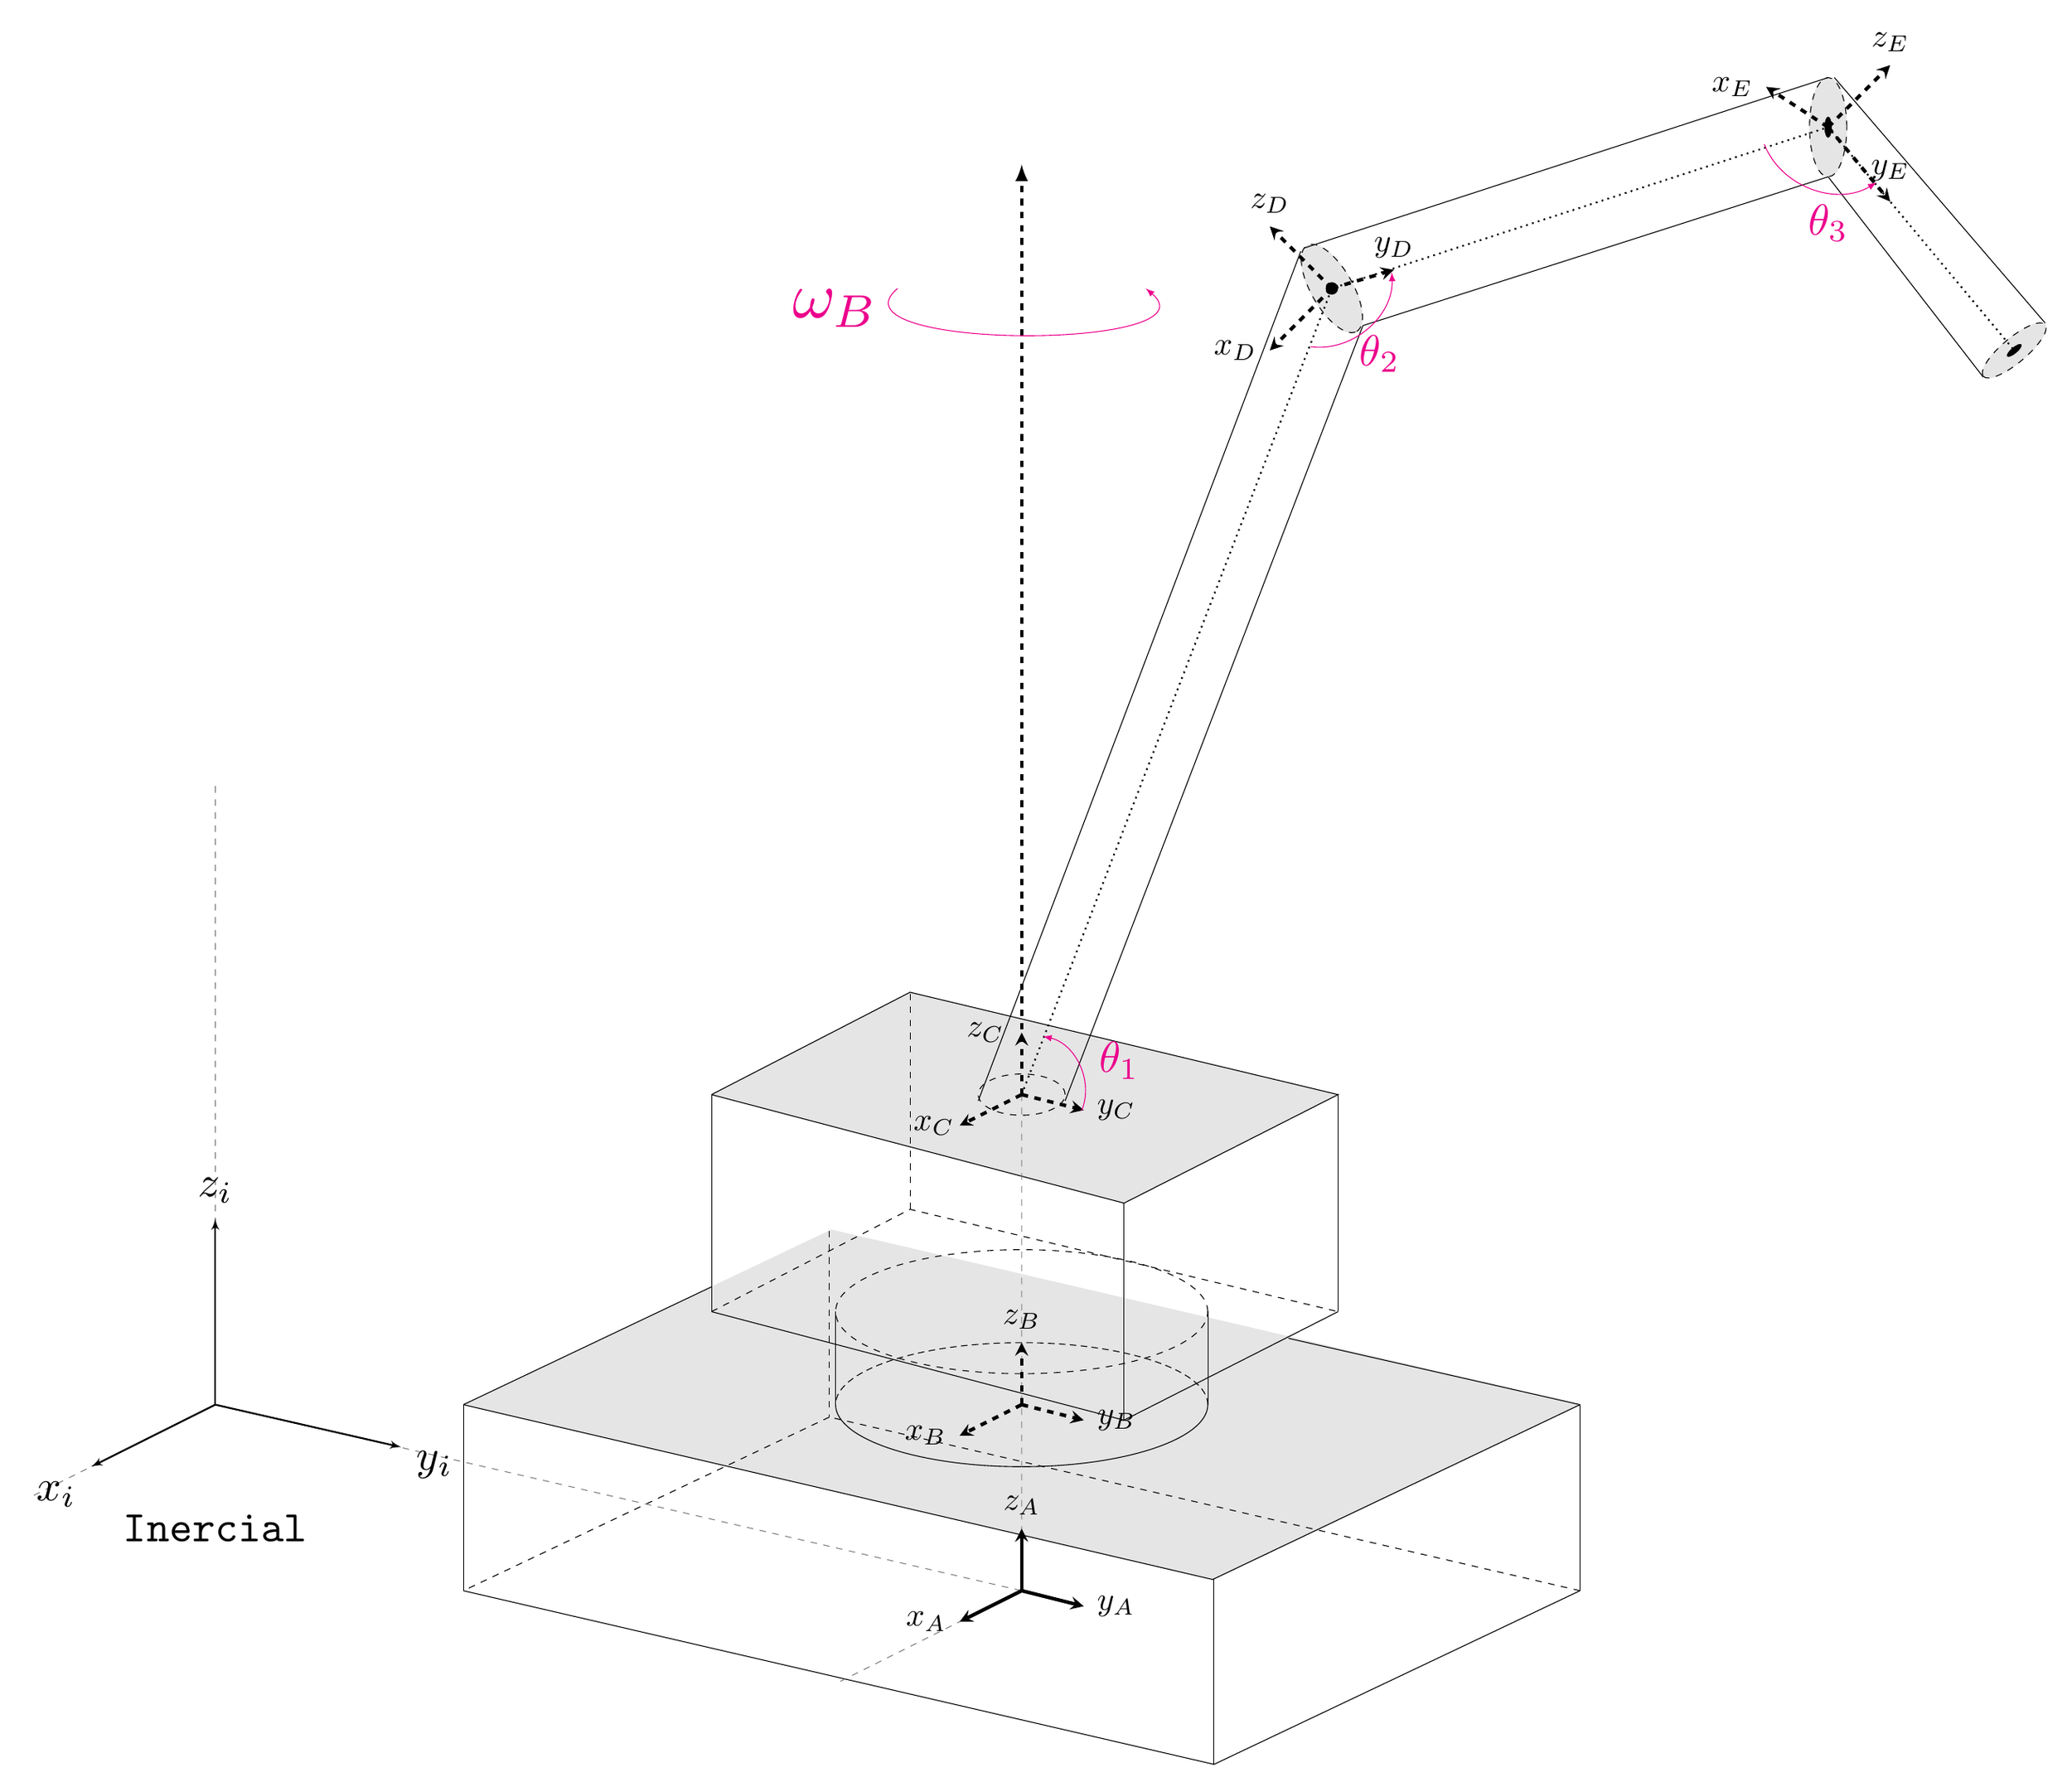
\begin{tikzpicture}[scale=1]
	\tkzDefPoints{0/0/O, 0/1.5/O', -3/0/A, 3/0/C, 0/5/A'}
	\coordinate (B) at (-70:3cm and 1cm);
	\tkzDefPointsBy[symmetry = center O](B){D}

	\tkzDefPointsBy[homothety = center O ratio 3](A,B,C,D){A1,B1,C1,D1}
	\tkzDefPointsBy[translation = from O to O'](A,B,C,D,A1,B1,C1,D1){F,G,H,E,F1,G1,H1,E1}
	
	\filldraw[gray!20] (A1) -- (B1) -- (C1) -- (D1);
	\draw (A1) -- (B1) -- (C1);
	\draw (A1) -- (-5,1.9);
	\draw (C1) -- (4.3,1.07);
	
	% Ellipse
	\filldraw[gray!20,rotate around={300:(5,18)}] (5,18) ellipse (.8cm and 0.333cm);
	\filldraw[gray!20] (13,20.6) ellipse (.3cm and .8cm);
	\filldraw[gray!20,rotate around={220:(16,17)}] (16,17) ellipse (.65cm and 0.2cm);
	
	\draw[densely dashed] (C) arc (0:180:3cm and 1cm);
	\draw (C) arc (0:-180:3cm and 1cm);
	\draw[dashed] (O') ellipse (3cm and 1cm);
	
	\tkzDrawPolySeg(A,F)
	\tkzDrawPolySeg(C,H)
	
	\draw[dashed](-5,1.5) -- (-1.8,3.15) -- (5.1,1.5);
	\draw (5.1,1.5) -- (1.65,-.25) -- (-5,1.5);
	
	% Quinas da base inferior
	\tkzDefPoints{-9/0/P1, 3.1/-2.8/P2, 9/0/P3, -3.1/2.8/P4}
	\draw (P1) -- (-9,-3);
	\draw (P2) -- (3.1,-5.8);
	\draw (P3) -- (9,-3);
	\draw[dashed] (P4) -- (-3.1,-0.2);
	
	% Retângulo inferior da base
	\draw (-9,-3) -- (3.1,-5.8) -- (9,-3);
	\draw[dashed] (-3.1,-.2) -- (-9,-3);
	\draw[dashed] (9,-3) -- (-3.1,-.2);
	
	% Tampa
	\filldraw[gray!20 ] (-5,5)--(-1.8,6.65)--(5.1,5)--(1.65,3.25) -- (-5,5);
	\draw (-5,5)--(-1.8,6.65)--(5.1,5)--(1.65,3.25) -- (-5,5);
	
	% Arestas laterais da cabine
	\draw (-5,1.5) -- (-5,5);
	\draw[dashed] (-1.8,3.15) -- (-1.8,6.65);
	\draw (5.1,1.5) -- (5.1,5);
	\draw (1.65,-.25) -- (1.65,3.25);
	
	% Referência
	\fill[black] (5,18) circle (1mm);
	\fill[black] (13,20.6) ellipse (.6mm and 1.7mm);
	\fill[black,rotate around={220:(16,17)}] (16,17) ellipse (1.5mm and .5mm);
	
	% Braço
	\draw[thick,dotted] (0,5) -- (5,18) -- (13,20.6) -- (16,17);
	
	% Braço - Trecho 1
	\draw[dashed] (0,5) ellipse (.7cm and 0.333cm);
	\draw (.7,4.9) -- (5.5,17.4);
	\draw (-.7,4.9) -- (4.5,18.6);
	
	% Braço - Trecho 2
	\draw[dashed,rotate around={300:(5,18)}] (5,18) ellipse (.8cm and 0.333cm);
	\draw (5.5,17.4) -- (13,19.8);
	\draw (4.55,18.65) -- (13,21.4);
	
	% Braço - Trecho 3
	\draw[dashed] (13,20.6) ellipse (.3cm and .8cm);
	
	% Ponta
	\draw[dashed,rotate around={220:(16,17)}] (16,17) ellipse (.65cm and 0.2cm);
	\draw (13,19.8) -- (15.5,16.57);
	\draw (13.1,21.4) -- (16.5,17.44);
	
	%%%%%%%%%%%%%%%%%%%%%%%%%%%%%%%%%%%%%%%%%%%%%%%%%%%%%%%%%%%%%%%%%%%%%%%%%%%%%%%%%
	
	% Eixos 
	\draw[dashed,gray] (0,5) -- (0,-3) -- (-13,0) -- (-13,10);
	\draw[dashed,gray] (-13,0) -- (-16,-1.5);
	\draw[dashed,gray] (0,-3) -- (-3,-4.5);
	
	\draw[->,>=latex',thick] (-13,0) -- (-10,-0.685);
	\draw[->,>=latex',thick] (-13,0) -- (-15,-1);
	\draw[->,>=latex',thick] (-13,0) -- (-13,3);
	\draw (-13,-2) node[scale=2]{\texttt{Inercial}};
	
	% Rótulos
	\draw (-10,-.5) node[scale=2,below right]{$y_{i}$};
	\draw (-15,-1) node[scale=2,below left]{$x_{i}$};
	\draw (-13,3) node[scale=2,above]{$z_{i}$};
	
	%%%%%%%%%%%%%%%%%%%%%%%%%%%%%%%%%%%%%%%%%%%%%%%%%%%%%%%%%%%%%%%%%%%%%%%%%%%%%%
	
	% Ponto A
	\draw[->,ultra thick, black,>=stealth] (0,-3) -- (0,-2) node[scale=1.5,above]{$z_{A}$};
	\draw[->,ultra thick, black,>=stealth] (0,-3) -- (1,-3.25) node[scale=1.5,right]{$y_{A}$};
	\draw[->,ultra thick, black,>=stealth] (0,-3) -- (-1,-3.5) node[scale=1.5,left]{$x_{A}$};
	
	% Ponto B
	\draw[->,ultra thick, black,>=stealth,dashed] (0,0) -- (0,1) node[scale=1.5,above]{$z_{B}$};
	\draw[->,ultra thick, black,>=stealth,dashed] (0,0) -- (1,-.25) node[scale=1.5,right]{$y_{B}$};
	\draw[->,ultra thick, black,>=stealth,dashed] (0,0) -- (-1,-.5) node[scale=1.5,left]{$x_{B}$};
	
	% Ponto C
	\draw[->,ultra thick, black,>=stealth,dashed] (0,5) -- (0,6);
	\draw (-.1,6) node[scale=1.5, left]{$z_{C}$};
	
	\draw[->,ultra thick, black,>=stealth,dashed] (0,5) -- (1,4.75) node[scale=1.5,right]{$y_{C}$};
	
	\draw[->,ultra thick, black,>=stealth,dashed] (0,5) -- (-1,4.50);
	\draw (-.9,4.5) node[scale=1.5,left]{$x_{C}$};
	
	% Ponto D
	\draw[->,ultra thick, black,>=stealth,dashed] (5,18) -- (6,18.3);
	\draw (6,18.3) node[scale=1.5, above]{$y_{D}$};
	
	\draw[->,ultra thick, black,>=stealth,dashed] (5,18) -- (4,19) node[scale=1.5,above]{$z_{D}$};
	
	\draw[->,ultra thick, black,>=stealth,dashed] (5,18) -- (4,17) node[scale=1.5,left]{$x_{D}$};
	
	% Ponto E
	% Ponto D
	\draw[->,ultra thick, black,>=stealth,dashed] (13,20.6) -- (14,19.4);
	\draw (14,19.55) node[scale=1.5, above]{$y_{E}$};
	
	\draw[->,ultra thick, black,>=stealth,dashed] (13,20.6) -- (14,21.6) node[scale=1.5,above]{$z_{E}$};
	
	\draw[->,ultra thick, black,>=stealth,dashed] (13,20.6) -- (12,21.25) node[scale=1.5,left]{$x_{E}$};
	
	% Ângulos
	\coordinate (A2) at (0,5);
	\coordinate (B2) at (5,18);
	\coordinate (F2) at (0,18);
	\coordinate (E2) at (13,21.55);
	
	
	\draw[->,>=latex,magenta] ([shift=(-15:1)]A2) to[bend right=50] ([shift=(70:1)]A2);
	\draw (1,5) node[magenta,scale=2,above right]{$\theta_{1}$};
	
	\draw[->,>=latex,magenta] ([shift=(250:1)]B2) to[bend right=50] ([shift=(15:1)]B2);
	\draw (5.2,16.4) node[magenta,scale=2,above right]{$\theta_{2}$};
	
	\draw[->,>=latex,magenta] ([shift=(230:1.6)]E2) to[bend right=50] ([shift=(293:2)]E2);
	\draw (13,19.6) node[magenta,scale=2,below]{$\theta_{3}$};
	
	\draw[->,dashed,>=latex,ultra thick] (0,5) -- (0,20);
	\draw[->,>=latex,magenta] ([shift=(180:2)]F2) to[bend right=140] ([shift=(0:2)]F2);
	\draw (-3,17) node[above,scale=3,magenta]{$\omega_{B}$};
	\end{tikzpicture}
	
	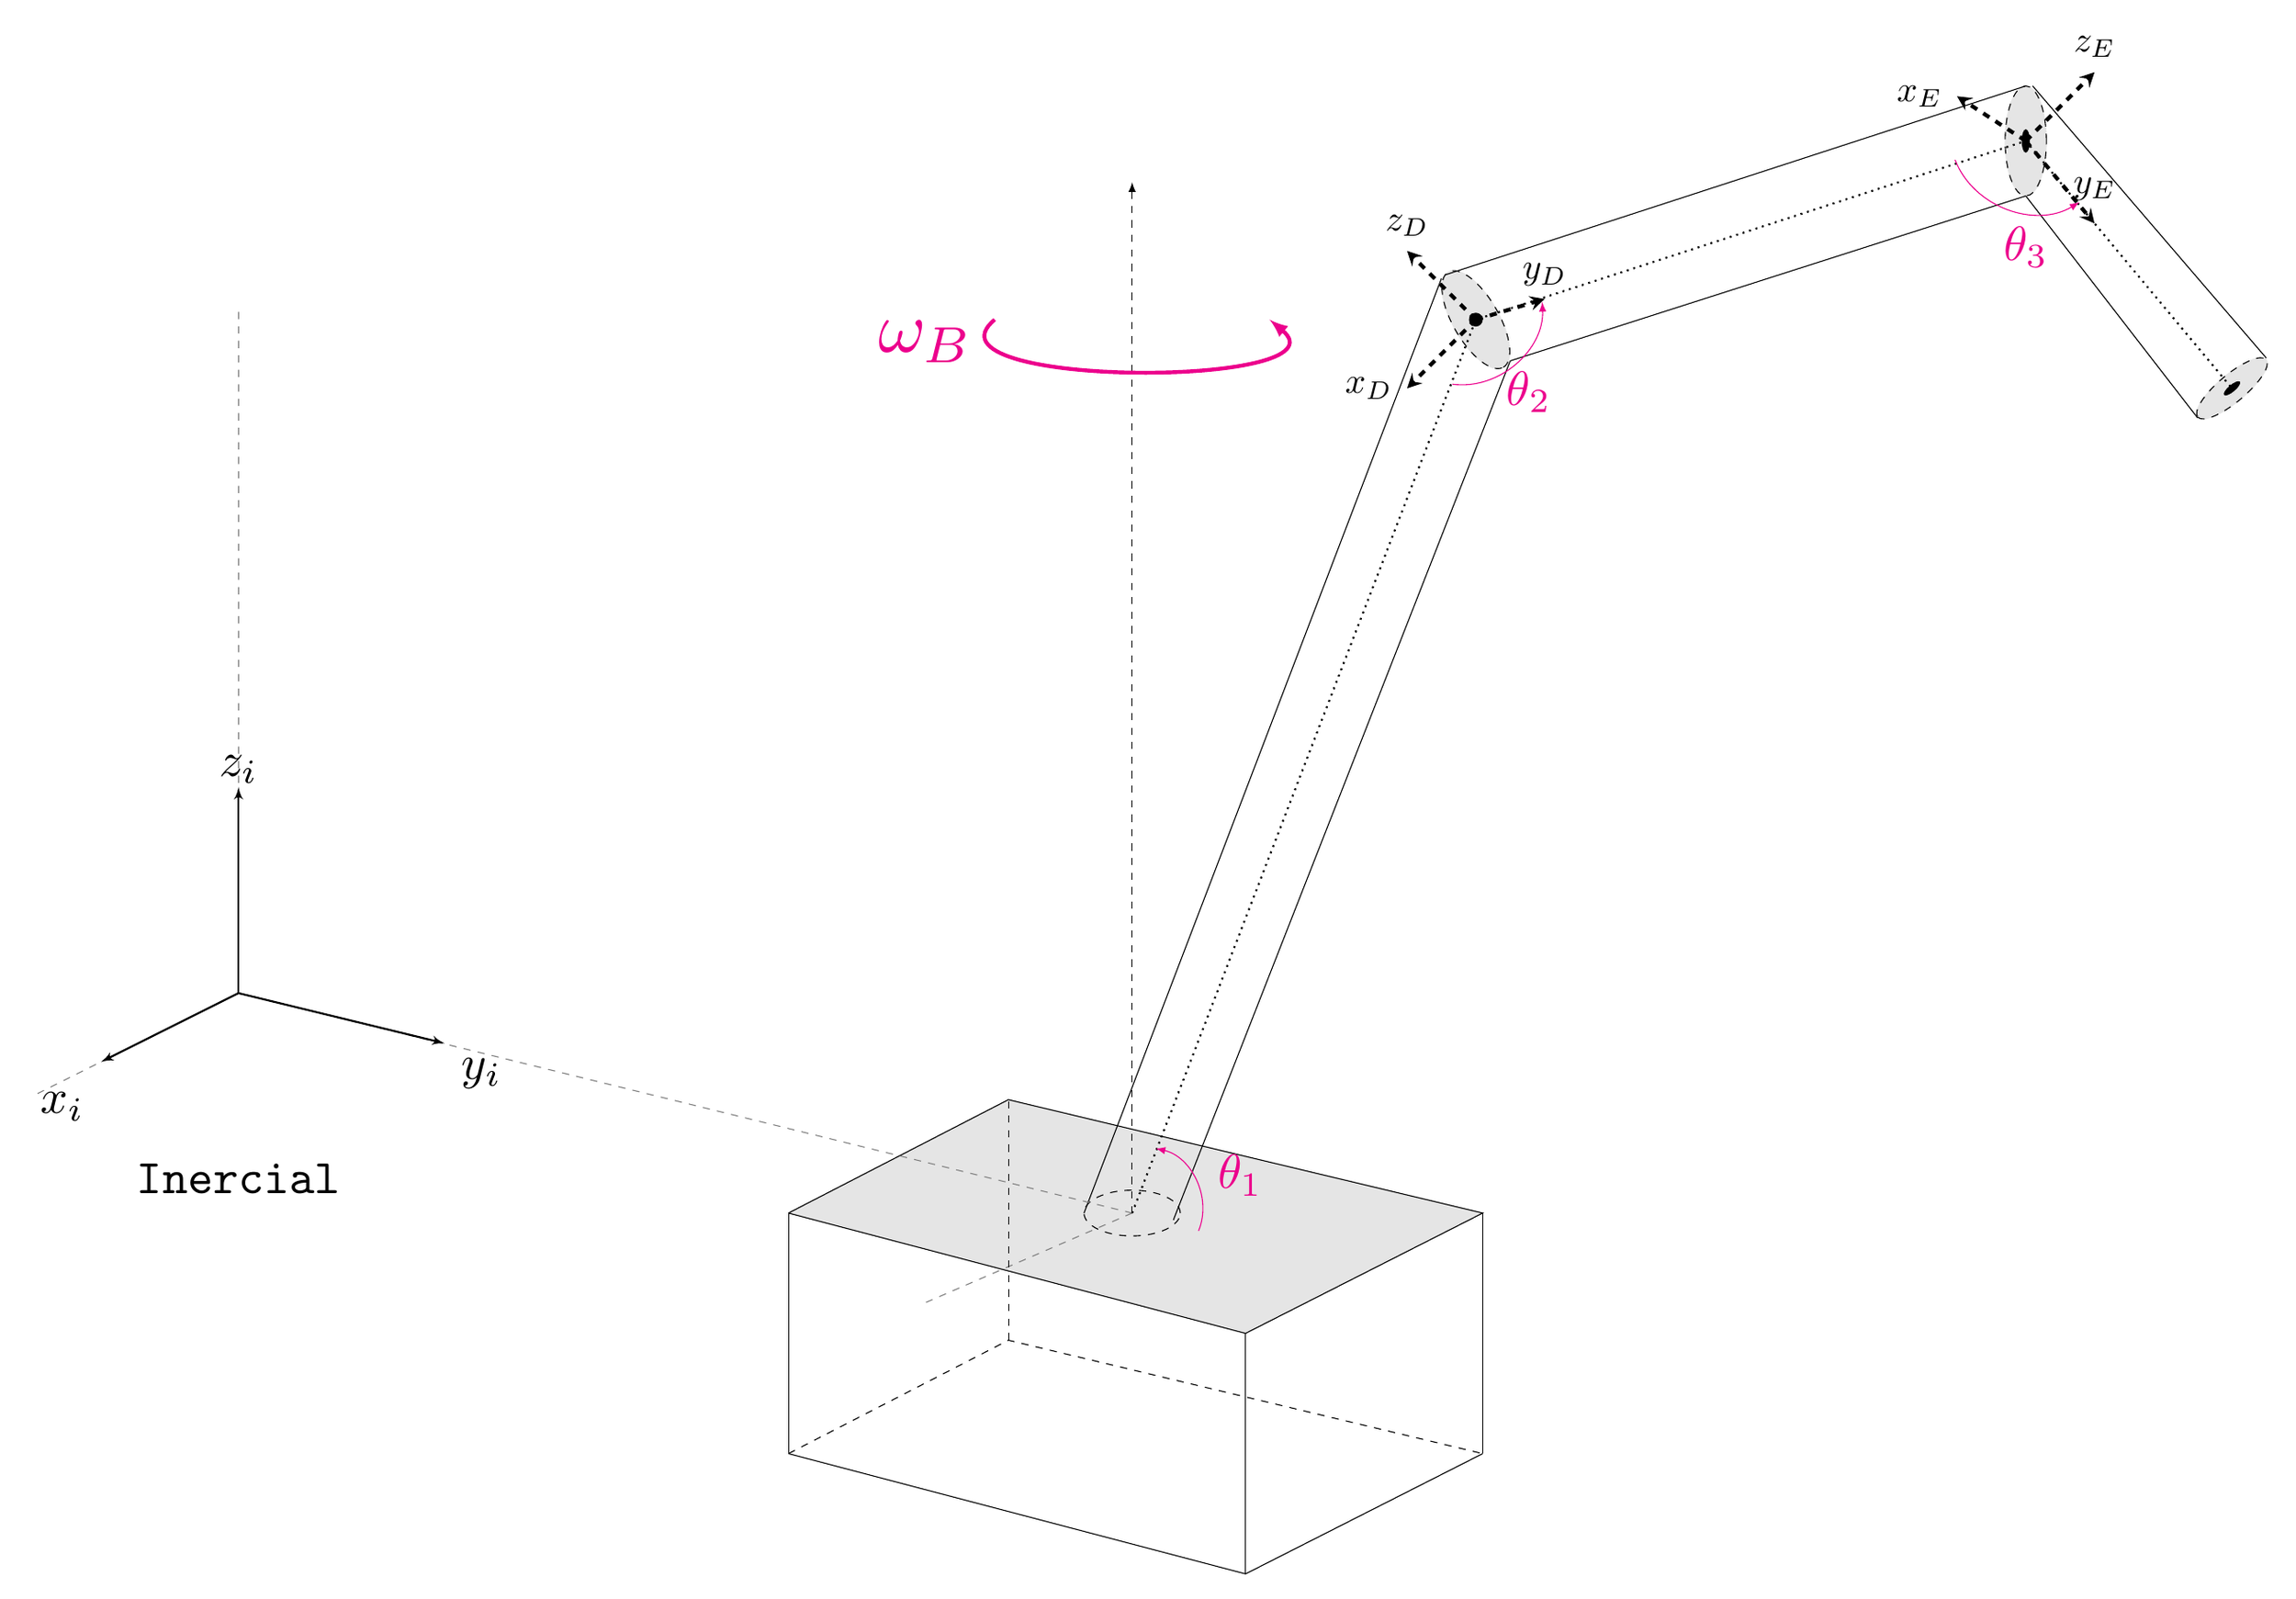
\begin{tikzpicture}[scale=1]
	\tkzDefPoints{0/0/O, 0/1.5/O', -3/0/A, 3/0/C, 0/5/A'}
	\coordinate (B) at (-70:3cm and 1cm);
	\tkzDefPointsBy[symmetry = center O](B){D}
	
	\tkzDefPointsBy[homothety = center O ratio 3](A,B,C,D){A1,B1,C1,D1}
	\tkzDefPointsBy[translation = from O to O'](A,B,C,D,A1,B1,C1,D1){F,G,H,E,F1,G1,H1,E1}
	
	% Ellipse
	\filldraw[gray!20,rotate around={300:(5,18)}] (5,18) ellipse (.8cm and 0.333cm);
	\filldraw[gray!20] (13,20.6) ellipse (.3cm and .8cm);
	\filldraw[gray!20,rotate around={220:(16,17)}] (16,17) ellipse (.65cm and 0.2cm);
	
	% Referência
	\fill[black] (5,18) circle (1mm);
	\fill[black] (13,20.6) ellipse (.6mm and 1.7mm);
	\fill[black,rotate around={220:(16,17)}] (16,17) ellipse (1.5mm and .5mm);
	
	\filldraw[gray!20 ] (-5,5)--(-1.8,6.65)--(5.1,5)--(1.65,3.25) -- (-5,5);
	\draw (-5,5)--(-1.8,6.65)--(5.1,5)--(1.65,3.25) -- (-5,5);
	
	% Braço
	\draw[thick,dotted] (0,5) -- (5,18) -- (13,20.6) -- (16,17);
	
	% Braço - Trecho 1
	\draw[dashed] (0,5) ellipse (.7cm and 0.333cm);
	\draw (.6,4.9) -- (5.5,17.4);
	\draw (-.7,5) -- (4.5,18.6);
	
	% Braço - Trecho 2
	\draw[dashed,rotate around={300:(5,18)}] (5,18) ellipse (.8cm and 0.333cm);
	\draw (5.5,17.4) -- (13,19.8);
	\draw (4.55,18.65) -- (13,21.4);
	
	% Braço - Trecho 3
	\draw[dashed] (13,20.6) ellipse (.3cm and .8cm);
	
	% Ponta
	\draw[dashed,rotate around={220:(16,17)}] (16,17) ellipse (.65cm and 0.2cm);
	\draw (13,19.8) -- (15.5,16.57);
	\draw (13.1,21.4) -- (16.5,17.44);
	
	%%%%%%%%%%%%%%%%%%%%%%%%%%%%%%%%%%%%%%%%%%%%%%%%%%%%%%%%%%%%%%%%%%%%%%%%%%%%%%%%%
	
	% Eixos 
	\draw[dashed,gray] (0,-3.2+4.5+.2+3.5) -- (-13,0+4.5+.2+3.5) -- (-13,10+4.5+.2+3.5);
	\draw[dashed,gray] (-13,0+4.5+.2+3.5) -- (-16,-1.5+4.5+.2+3.5);
	\draw[dashed,gray] (0,-3.2+4.5+.2+3.5) -- (-3,-4.5+4.5+.2+3.5);
	
	\draw[->,>=latex',thick] (-13,0+4.5+.2+3.5) -- (-10,-0.73+4.5+.2+3.5);
	\draw[->,>=latex',thick] (-13,0+4.5+.2+3.5) -- (-15,-1+4.5+.2+3.5);
	\draw[->,>=latex',thick] (-13,0+4.5+.2+3.5) -- (-13,3+4.5+.2+3.5);
	\draw (-13,-2+4+3.5) node[scale=2]{\texttt{Inercial}};
	
	% Rótulos
	\draw (-10,-.5+4.5+3.5) node[scale=2,below right]{$y_{i}$};
	\draw (-15,-1+4.5+3.5) node[scale=2,below left]{$x_{i}$};
	\draw (-13,3+4.5+3.5) node[scale=2,above]{$z_{i}$};
	
	%%%%%%%%%%%%%%%%%%%%%%%%%%%%%%%%%%%%%%%%%%%%%%%%%%%%%%%%%%%%%%%%%%%%%%%%%%%%%%
	
	% Ponto D
	\draw[->,ultra thick, black,>=stealth,dashed] (5,18) -- (6,18.3);
	\draw (6,18.3) node[scale=1.5, above]{$y_{D}$};
	
	\draw[->,ultra thick, black,>=stealth,dashed] (5,18) -- (4,19) node[scale=1.5,above]{$z_{D}$};
	
	\draw[->,ultra thick, black,>=stealth,dashed] (5,18) -- (4,17) node[scale=1.5,left]{$x_{D}$};
	
	% Ponto D
	\draw[->,ultra thick, black,>=stealth,dashed] (13,20.6) -- (14,19.4);
	\draw (14,19.55) node[scale=1.5, above]{$y_{E}$};
	
	\draw[->,ultra thick, black,>=stealth,dashed] (13,20.6) -- (14,21.6) node[scale=1.5,above]{$z_{E}$};
	
	\draw[->,ultra thick, black,>=stealth,dashed] (13,20.6) -- (12,21.25) node[scale=1.5,left]{$x_{E}$};
	
	% Ângulos
	\coordinate (A2) at (0,5);
	\coordinate (B2) at (5,18);
	\coordinate (F2) at (0,18);
	\coordinate (E2) at (13,21.55);
	
	
	\draw[->,>=latex,magenta] ([shift=(-15:1)]A2) to[bend right=50] ([shift=(70:1)]A2);
	\draw (1,5) node[magenta,scale=2,above right]{$\theta_{1}$};
	
	\draw[->,>=latex,magenta] ([shift=(250:1)]B2) to[bend right=50] ([shift=(15:1)]B2);
	\draw (5.2,16.4) node[magenta,scale=2,above right]{$\theta_{2}$};
	
	\draw[->,>=latex,magenta] ([shift=(230:1.6)]E2) to[bend right=50] ([shift=(293:2)]E2);
	\draw (13,19.6) node[magenta,scale=2,below]{$\theta_{3}$};
	
	\draw[->,dashed,>=latex] (0,5) -- (0,20);
	
	\draw[->,>=latex,magenta,ultra thick] ([shift=(180:2)]F2) to[bend right=140] ([shift=(0:2)]F2);
	\draw (-3,17) node[above,scale=3,magenta]{$\omega_{B}$};

	%Arestas laterais da cabine
	\draw (-5,1.5) -- (-5,5);
	\draw[dashed] (-1.8,3.15) -- (-1.8,6.65);
	\draw (5.1,1.5) -- (5.1,5);
	\draw (1.65,-.25) -- (1.65,3.25);
	
	\draw[dashed](-5,1.5) -- (-1.8,3.15) -- (5.1,1.5);
	\draw (5.1,1.5) -- (1.65,-.25) -- (-5,1.5);
	\end{tikzpicture}
\end{document}
